%
% $Id: ch01_overview
%
%   *******************************************************************
%   * SEE THE MAIN FILE "AllegThesis.tex" FOR MORE INFORMATION.       *
%   *******************************************************************

\chapter{Introduction}
\label{ch:intro}

In the early days of computing, real-time rendering engines that powered games like {\it Doom} or {\it NetHack} had to run on extremely underpowered hardware and render on low-resolution screens.
The dream of real-time, photorealistic graphics was far, far away.
However, even then the simple, blocky graphics, easily recognizable shapes, and maze-like environments were fantastic entertainment.
Today the retro-style of low-resolution graphics, pixel art, and 8-bit color is abound in the gaming space.
This proposal is one part of enabling that retro-aesthetic to grow into a new and unique style that, while similar to the old classics, can be more engaging and real than they ever were.
With the current generation of powerful CPU and GPU chips, able to execute billions and trillions of calculations per second respectively, it is finally possible to do real-time, close to photorealistic rendering.
While the goal of \name\ is not high-resolution photorealism, some approximation of photorealism will be obtained, albeit at a lower resolution.

\section{Overview}
\label{ch:intro:overview}

This thesis document describes \name, a system that creates a moving image on a terminal screen.
This rendering engine performs real-time updating of the displayed image, generating an animation.
\name\ uses the recursive ray-tracing algorithm, simulating the path of light through the scene -- this is described in more detail in Section~\ref{ch:intro:overview:raytracing}.
Rendered images are displayed in two different modes; the first uses single half-character pixels, and the second more complex Unicode block characters.
The mechanics of this image composition method are discussed in Section~\ref{ch:intro:overview:unicode}.
Once an image is rendered, the \texttt{ncurses} C library \cite{ncursesLibrary} is used to display it in a terminal.
An example of the final terminal output is Figure~\ref{fig:checker_metal}, which was generated by TerminalImageViewer \cite{tivGithub} as a mockup \inlinetodo{this should be an actual output image, and described as such}.
More details on this process are given in Section~\ref{ch:intro:overview:ncurses}.

\begin{figure}[htb]
  \centering
  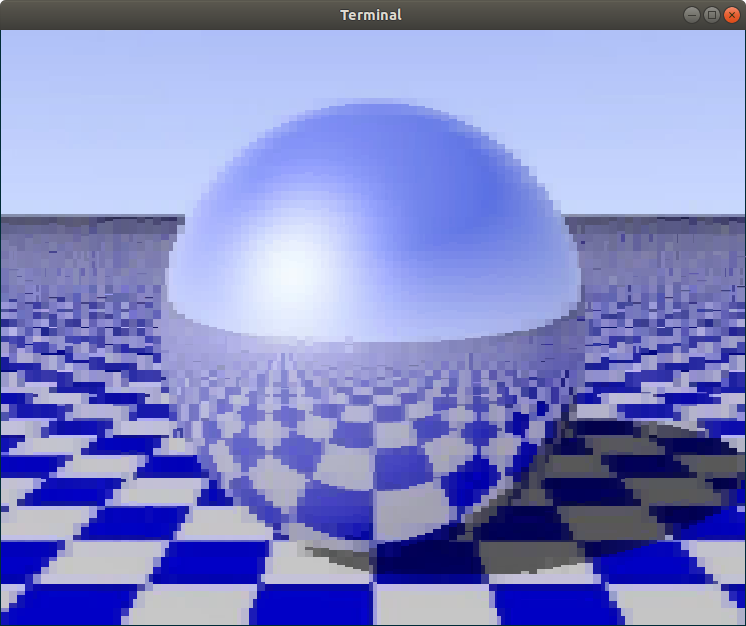
\includegraphics[width=0.8\textwidth]{resources/checker_metal}
  \caption{Example of proposed terminal output}
  \label{fig:checker_metal}
\end{figure}

\subsection{Rendering Engines and Ray-Tracing}
\label{ch:intro:overview:raytracing}

A rendering engine is an algorithm that takes a scene -- a description of some collection of objects -- and generates an image or visual representation of that scene.
There are many different algorithms that accomplish this goal.
In this proposal, the recursive ray-tracing algorithm first pioneered by Turner Whitted in his ground-breaking paper {\it An Improved Illumination Model for Shaded Display} \cite{whitted1980improved}, will be discussed and utilized.
Ray-tracing was one of the first algorithms developed in the field of computer graphics, and although there have been some improvements since then, the idea behind the algorithm has maintained its original simplicity.

Ray-tracing has been used as the renderer of choice for photorealistic images, because with only a few modifications to Whitted's original algorithm, it can generate fantastic images.
In the past, however, render times have been so slow that it was impossible to generate images fast enough for real-time use.
For example, Figure~\ref{fig:povray_render} is a render created by the POV-Ray engine \cite{povray}.
POV-Ray can take between a few minutes to several hours to complete one single image depending on the processing power involved.
However, there have been a few recent innovations that change this, such as NVIDIA's RTX hardware acceleration.
Section~\ref{ch:intro:background:hardware} provides more details on these advances, as well as an explanation of how ray-tracing will be utilized in \name.

\begin{figure}[htb]
  \centering
  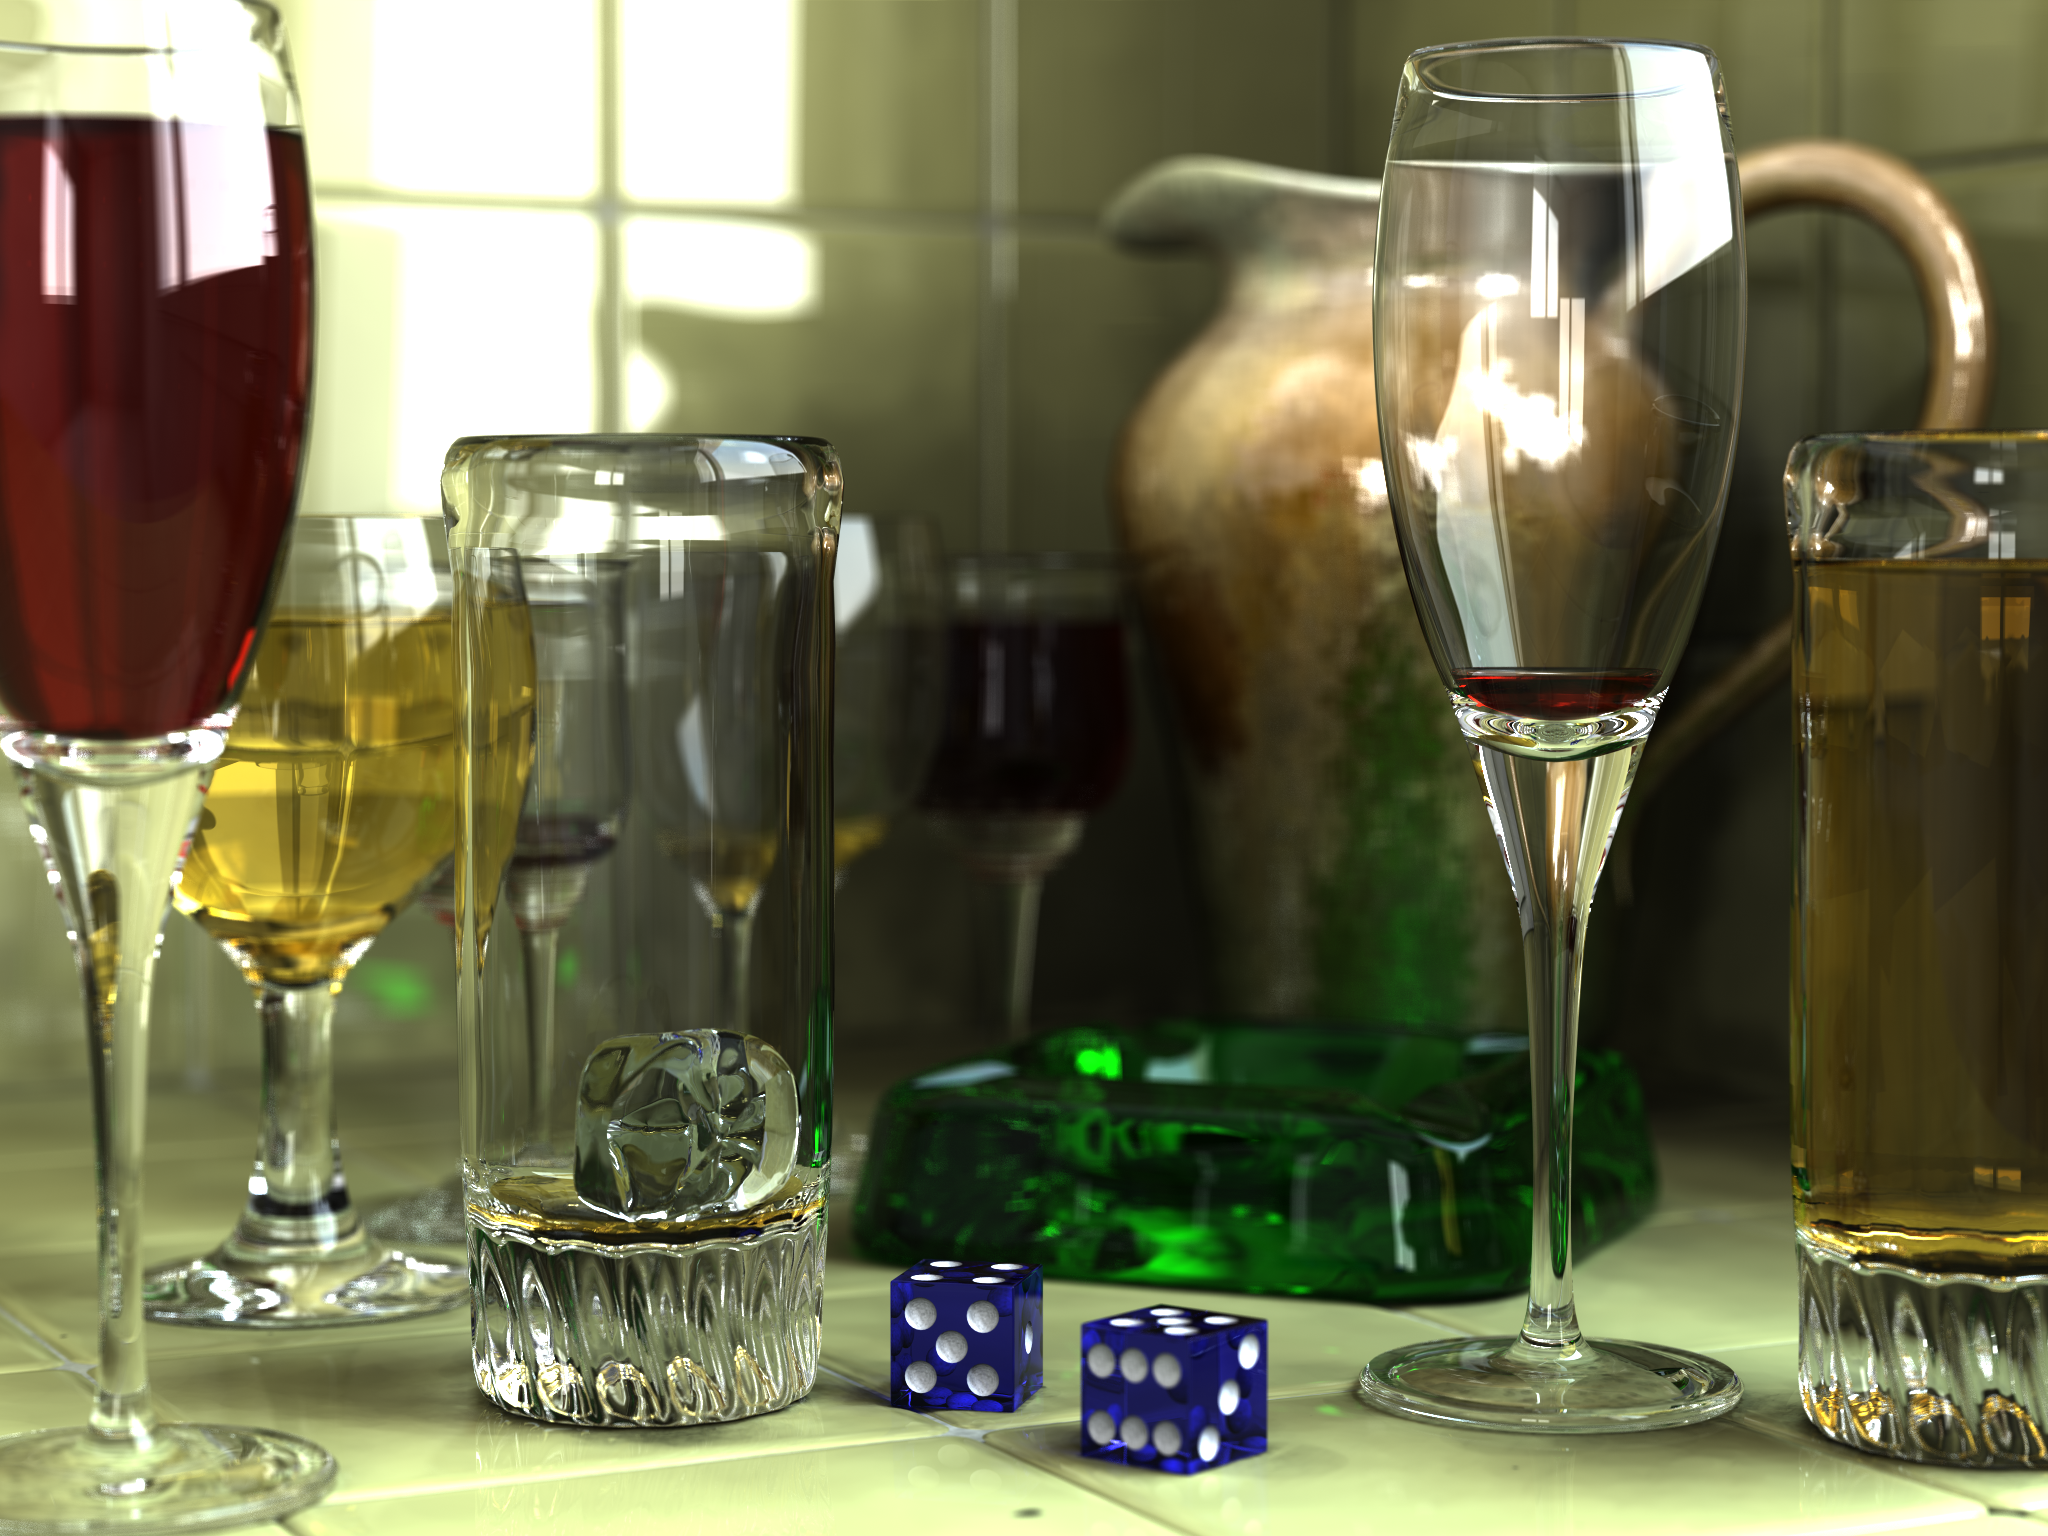
\includegraphics[width=0.8\textwidth]{resources/glasses_povray}
  \caption{POV-Ray render created by Gilles Tran \cite{povray2006render}}
  \label{fig:povray_render}
\end{figure}


Ray-tracing revolves around the idea of {\it rays}, a mathematical construct which can be defined by two vectors: an origin point, referred to as $\rayorg$ for some ray $R$, and a direction, referenced as $\raydir$.
These two vectors together represent a ray of infinite length that starts at the origin and projects along the direction.
An important addition to the concept of rays is a point along a ray -- this can be defined by using a third variable, $t$, to represent how far along the ray the point is located.
Therefore, Formula~\ref{equation:point_on_ray} can be used to get the coordinates of a point in three-dimensional space (assuming $\raydir$ is a unit vector).
This is called the {\it parametric~form} of a ray.
The mathematics behind ray-tracing are further explored in Section~\ref{ch:intro:background}.

\begin{equation}
  \label{equation:point_on_ray}
  \vec{point} = \rayorg + t\raydir
\end{equation}

In ray-tracing, rays are used to simulate the path that light takes as it travels around the scene.
When a ray intersects with an object in the scene various interactions take place that simulate how light may travel under different conditions.
It is worth noting that a base assumption is made in ray-tracing when using straight rays as described here: light follows a straight line without changes.
This is only the case in reality when light travels through a vacuum with no gravitational bodies; thus, basic ray-tracing is not exactly photorealistic and does not model phenomena like atmospheric scattering.
Additional mathematics and systems must be used to bend, attenuate, or scatter a ray to accurately render transparent volumes -- this is called volumetric ray-tracing.
Volumetric ray-tracing will not be supported by the proposed \name, but would be a fascinating area of future work.

The basis for ray-tracing is the rendering equation, articulated by James Kajiya in 1986 \cite{kajiya1986rendering}.
The rendering equation models the outgoing light at some point given all incoming light, a bidirectional reflectance distribution function (BDRF), and a normal for the surface at the point modeled.
If solved for every point in the scene, the rendering equation could generate a completely photorealistic image -- this would, however, require massive amounts of computation.
This is because the rendering equation contains an integral over all incoming light which must be solved through numerical analysis.
Ray-tracing engines that do this are known as {\it path-tracers} and are the most photorealistic rendering engines invented.

\name\ will not use a path-tracer -- such algorithms are still many times too slow for most real-time rendering situations.
Instead, the rendering equation will be solved by sampling the incoming light with rays.
This is known as recursive ray-tracing, since it starts with a single ray that splits every time it encounters a surface.
The eventual goal of the recursive ray-tracing algorithm is to create a tree of rays for each {\it fragment} to render.
A fragment is either a pixel or some sub-pixel -- many systems will use four or more fragments per pixel to get better anti-aliasing and more accurate results.
Each ray contains some color that represents the color of the light in that ray.
When a ray hits an object, it is {\it scattered} by the {\it material} of the object, splitting and generating new rays.
These rays are biased towards directions that contain lots of incoming light -- such as towards a point light source.
The specific implementation of recursive ray-tracing that \name\ will use will only scatter into a set number of rays at each intersection point: one ray toward each light source, along with reflection and refraction rays towards the relevant directions.

The base of each generated tree is an {\it eye-ray} -- a ray with its origin at the fragment location on the camera plane.
The eye-ray's color is the color that will be rendered for that fragment.
As the eye-ray projects forward, away from the eye, it is tested for intersection with all objects in the scene.
When an intersection happens and the generated rays scattered, the eventual color values of the scattered rays are combined to produce the color of the original eye-ray.
This is done recursively to fully render the scene.


\subsection{Image Composition using Unicode Characters}
\label{ch:intro:overview:unicode}

Unicode is a character standard that allows anyone to reference many thousands of characters to compose text, no matter the environment around the text \cite{unicode}.
Some critical characters that \name\ will use are known as the {\it block characters} -- they are characters \texttt{U+2580} -- \texttt{U+259F}.
Relevant characters are shown in Figure~\ref{fig:unicode_characters}.
Contingent on the quality of the output using only block characters, additional sets could be used, such as triangles and lines.
The core of image composition using Unicode is an algorithm coloring the characters and the background -- \name\ will use this algorithm on every character of the output to both determine the character to display, and the foreground and background colors for that character.
The foreground colors the character itself, whereas the background provides a relief color.
This allows each {\it character~pixel} to represent a hard gradient.

\begin{figure}[htb]
  \centering
  \hspace{0.3em}
  \begin{subfigure}[htb]{0.4\textwidth}
    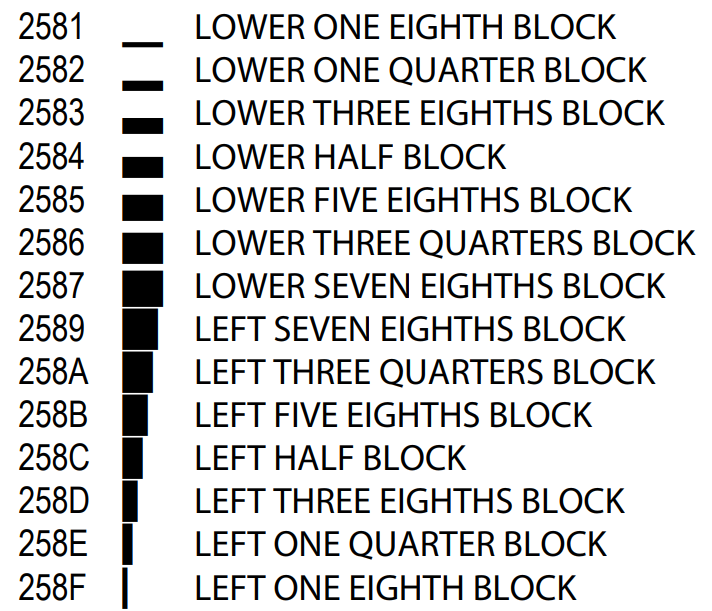
\includegraphics[width=\textwidth]{resources/block_elements}
    \caption{Block Elements}
    \label{fig:unicode_block_characters}
  \end{subfigure}
  \hfill
  \begin{subfigure}[htb]{0.51\textwidth}
    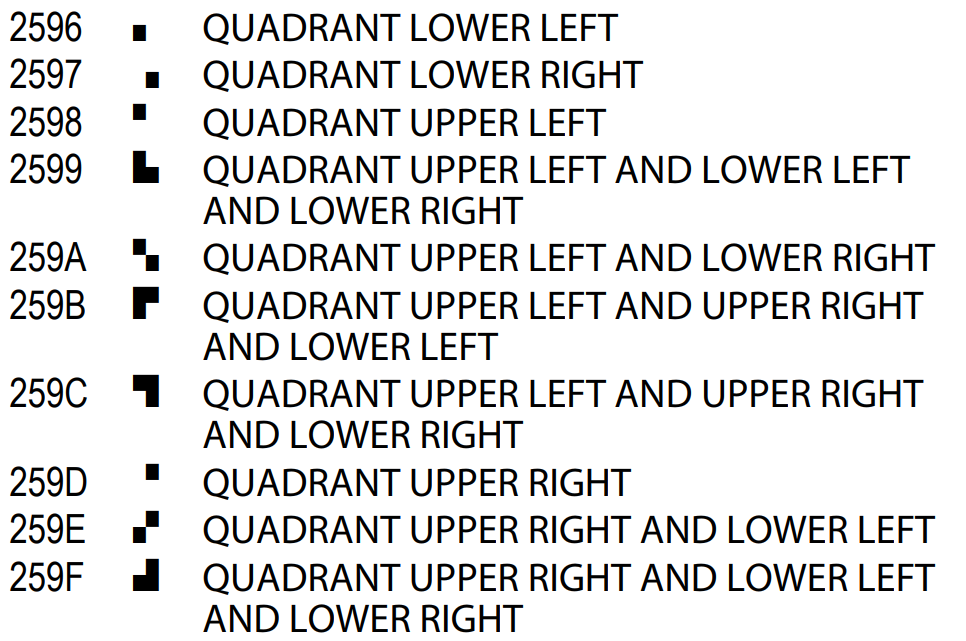
\includegraphics[width=\textwidth]{resources/quadrant_elements}
    \caption{Quadrant Elements}
    \label{fig:unicode_quadrant_characters}
  \end{subfigure}
  \caption{Subset of \texttt{U+2580} -- \texttt{U+259F} \cite{unicode}}
  \label{fig:unicode_characters}
\end{figure}

There are two image modes that will be available for use in \name.
The first is pure {\it pixel mode}, in which the Unicode ``half-block'' symbol (\texttt{U+2584}) is used.
Since mono-spaced character output (such as in a terminal) is twice as tall as it is wide, the half-block can split a single character into two pixels that are colored differently: the upper pixel with the background color of the character, and the lower with the character or foreground color of the pixel.
This would mean that a typical 85 by 30 character terminal would result in a screen space of 85 by 60 pixels.
This mode also dramatically reduces the number of ray-tracing computations needed, since only one ray per pixel is required.

The second image mode is considerably more complicated and slower, as it uses significantly more rays per character in order to determine what Unicode block character most fits the desired output.
On the other hand, it allows a much higher perceived resolution, since the characters used have smaller footprints of down to an eigth of a character in width or length.
The differences between these two modes are highlighted in Figure~\ref{fig:unicode_mode_comparison1} and~\ref{fig:unicode_mode_comparison2}.
It can be seen that the first image mode, {\it pixel mode}, shows a rather fuzzy definition of the main large sphere.
However, in the second image mode, {\it character mode}, the sphere and the reflections seen in it are much more defined.
The performance impact of both modes is another factor that must be assessed when making implementation decisions for \name.

\begin{figure}[htb]
  \centering
  \begin{subfigure}[htb]{0.49\textwidth}
    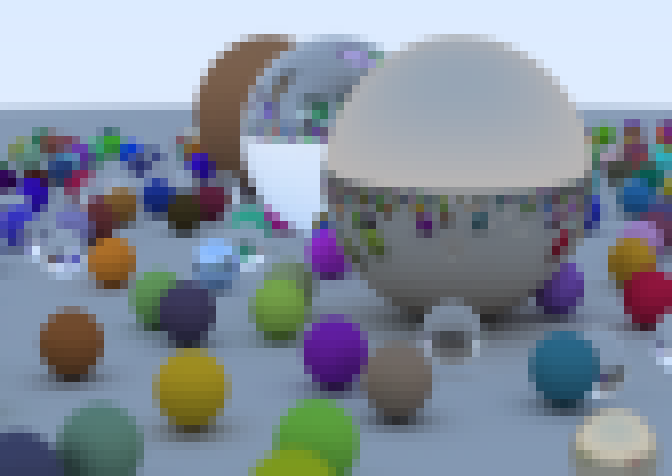
\includegraphics[width=\textwidth]{resources/many_spheres_square}
    \caption{Pixel Mode Image Output}
    \label{fig:unicode_mode_comparison1}
  \end{subfigure}
  \hfill
  \begin{subfigure}[htb]{0.49\textwidth}
    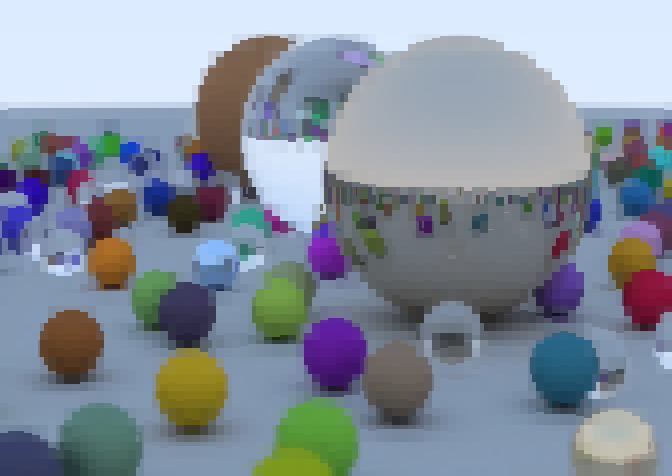
\includegraphics[width=\textwidth]{resources/many_spheres}
    \caption{Character Mode Image Output}
    \label{fig:unicode_mode_comparison2}
  \end{subfigure}
  \caption{Examples of Image Mode Output}
  \label{fig:unicode_mode_comparison}
\end{figure}

\subsection{Terminal Output using \texttt{ncurses}}
\label{ch:intro:overview:ncurses}

Once an image is generated, \name\ must somehow display that image in a terminal with no surrounding prompt or other formatting -- just a simple {\it character field}.
To do this, we will use \texttt{ncurses}, a C library that abstracts implementation details of the terminal to enable full-window 24-bit color character output.
Using \texttt{ncurses}, the terminal window will be divided into two ``panels'', a main panel for the actual image output -- updated 30 to 60 times per second -- and an info panel to render information such as frames per second and logging information.
With this dependency, \name\ can be used on all terminals that support \texttt{ncurses} -- generally, any XTerm-like terminal will work, as long as it supports a terminal information database: either \texttt{termcap} or \texttt{terminfo} will work.

A possible limitation to \texttt{ncurses} is keyboard input handling -- there is no mechanism to get events on an up or down movement of a key, as is possible in some other libraries.
Therefore, research will need to be done on possible alternatives for the input aspect of the engine.
This is not a priority, however, since it is not related to the rendering nature of \name and instead only helps with demonstrations of its capabilities.


\section{Background} \label{ch:intro:background}

The background information for the algorithms and techniques used to implement \name\ are discussed in this section.
In Section~\ref{ch:intro:background:algorithms} we detail most of the mathematics involved.
Software tools and languages utilized to build \name\ are discussed in Section~\ref{ch:intro:background:software}.
Finally, hardware interfaces, along with the current landscape of hardware availability, are covered in Section~\ref{ch:intro:background:hardware}.
Additionally, discussion on parallelization is presented.

\subsection{Algorithms and Mathematics}
\label{ch:intro:background:algorithms}
The mathematical basis for ray-tracing, which we describe later in this section, relies on an understanding of basic vector mathematics.
These algorithms will be running millions of times per second in a highly parallelized environment.
In this context, parallelization is a method of running two or more algorithm simultaneously; therefore even minor optimizations reduce the overall time to render, and are extremely important.
All of the ray-tracing mathematics described here are synthesized from Peter Shirley's excellent {\it Ray Tracing in One Weekend} \cite{shirley2016ray} and the Morgan Kaufmann textbook {\it Physically Based Rendering: From Theory to Implementation} \cite{pharr2016physically}.

Scenes that can be ray-traced must be a collection of surfaces that are mathematically intersectable with a ray.
Any surface that can be defined by a implicit surface definition function, in the form of Function~\ref{equation:surface_equation}, is intersectable with a ray \cite{pharr2016physically}.
In Function~\ref{equation:surface_equation} and for the rest of this section, $\vec{p}$ is a vector representing a point in three-dimensional space.
The implicit surface definition function must have the property that if and only if $f(\vec{p})$ is $0$, then $\vec{p}$ is on the defined surface.
The point of intersection between a ray and a surface defined in this way can be found by solving Equation~\ref{equation:ray_surface_intersection} for $t$ and then using Formula~\ref{equation:point_on_ray} to calculate the coordinates of that point on the ray.

\begin{equation}
  \label{equation:surface_equation}
  f(\vec{p}) = 0
\end{equation}

\begin{equation}
  \label{equation:ray_surface_intersection}
  f(\rayorg + t\raydir) = 0
\end{equation}

In \name, the only surfaces that are supported are spheres, triangles, and infinite planes, since their surface definition functions are mathematically simple.
If there is additional development time and resources available, other shapes such as quads, arbitrary polygons, and cubes may be considered.
This may not be a huge development effort, as the algorithm discussed for triangle intersection testing is applicable to any convex polygon.
A sphere is the simplest three-dimensional object to calculate ray intersection with, and therefore will be the first implemented for \name.
In fact, during feasibility testing much of the math described in this section was implemented in the Go programming language.

\littlesection{Ray-Sphere Intersection}

The surface definition function of a sphere is Function~\ref{equation:sphere_surface}, with $S$ representing the sphere.
The intersection point between a ray and a sphere is given by solving Equation~\ref{equation:ray_sphere_intersection} for $t$ and then using Formula~\ref{equation:point_on_ray}.
Both of these equations are directly adapted from {\it Ray Tracing in One Weekend} \cite{shirley2016ray}.
Notice that Equation~\ref{equation:ray_sphere_intersection} is quadratic, and the number (and values) of the roots give us the $t$ we want to use.
The smallest positive root corresponds to the point on the ray which first intersects the sphere.
If there are no real roots, then the ray does not intersect the sphere.

\begin{equation}
  \label{equation:sphere_surface}
  f(\vec{p}) = (\vec{p} - \vec{S_{center}})^2 - {S_{radius}}^2
\end{equation}

\begin{equation}
  \label{equation:ray_sphere_intersection}
  (\raydir^2)t^2 + 2(\raydir \cdot (\rayorg - \vec{S_{center}}))t + (\rayorg - \vec{S_{center}})^2 - {S_{radius}}^2 = 0
\end{equation}

\littlesection{Ray-Plane Intersection}

For any two-dimensional object, the plane it lies in is the first shape tested for intersection.
Luckily, ray-plane intersection testing is fairly cheap and straight forward.
The surface definition function of a plane is Function~\ref{equation:plane_surface}, with $P$ representing the plane.
The plane's {\it offset} is a point on the plane, and the plane's {\it normal} is a vector perpendicular to the plane.
The intersection point between a ray and a plane is given by solving Equation~\ref{equation:ray_plane_intersection} for $t$ and then using Formula~\ref{equation:point_on_ray}.
These equations were derived from basic vector math, along with guidance from {\it Physically Based Rendering} \cite{pharr2016physically}.

\begin{equation}
  \label{equation:plane_surface}
  f(\vec{p}) = (\vec{p} - \vec{P_{offset}}) \cdot \vec{P_{normal}}
\end{equation}

\begin{equation}
  \label{equation:ray_plane_intersection}
  (\vec{P_{normal}} \cdot \raydir)t + \vec{P_{normal}} \cdot (\rayorg - \vec{P_{offset}}) = 0
\end{equation}

\littlesection{Ray-Triangle Intersection}

The method for testing intersection with triangles is a bit more complicated than the other tests we've covered so far.
The mathematics for this section are again derived from vector mathematics.
However, Jean-Colas Prunier's {\it Scratchapixel}, an excellent and accessible online resource for 3D rendering \cite{prunier2017triangle}, was also an indispensable guide in facilitating understanding along the way.
First, intersection is tested with the plane the triangle lies in -- this results in a ray-plane intersection point $\vec{Q}$, or no intersection.
Then, if there was an intersection, another test must be performed to detect if $\vec{Q}$ is inside the triangle.
We do this using the ``inside-outside'' method (as suggested by {\it Scratchapixel}): test if $\vec{Q}$ is on the left side of each edge.

To conduct the left-side test, we label each triangle vertex $\vec{V_i}$, with $i$ increasing in the counter-clockwise direction.
We then have three triangle vertices: $\vec{V_0}$, $\vec{V_1}$, and $\vec{V_2}$.
We can now use Function~\ref{equation:left_edge_test}: if $f(i) > 0$ for each $i$, then $\vec{Q}$ is inside the triangle.
Otherwise, $\vec{Q}$ is outside the triangle.
Note that in Function~\ref{equation:left_edge_test}, if $i = 3$, then $i = 0$ ($i$ ``wraps'' to only valid values).

\begin{equation}
  \label{equation:left_edge_test}
  f(i) = P_{normal} \cdot ((\vec{V_{i+1}} - \vec{V_i}) \times (\vec{Q} - \vec{V_i}))
\end{equation}

Function~\ref{equation:left_edge_test} can be complicated to visualize, so imagine this: we first form two vectors, both with $\rayorg = \vec{V_i}$.
One points along the triangle's edge, while the other points to $\vec{Q}$.
Both of these vectors will be in the plane of the triangle.
Thus, if we cross them, the vector produced will either be away from the plane in the same direction as $\vec{P_{normal}}$, or away from the plane in the opposite direction.
According to the right hand rule, if the crossed vector is in the same direction as $\vec{P_{normal}}$, then the vector pointing to $\vec{Q}$ is ``to the left'' of the vector pointing towards $\vec{V_{i+1}}$.
We can then calculate the dot product between $\vec{P_{normal}}$ and the crossed vector -- if it is positive then the crossed vector is in the same direction as the normal, and therefore $\vec{Q}$ is to the left of the edge.
One last addendum to this intersection test is the fact that it can be difficult to perform the counter-clockwise numbering of vertices.
We will therefore simply expect vertices to be specified in counter-clockwise order.
This is similar to what many other 3D rendering programs assume.

\name's implementation will be hosted on Github, a public platform for projects using the Git version control system.
Travis CI \cite{travisci}, a continuous integration system, will be used for testing and environment management.
Documentation was handled by \texttt{doxygen} \cite{van2008doxygen} -- all external facing functions, methods, and classes will have a minimum of a few sentences of documentation.
More details about the implementation tools are given in Section~\ref{ch:intro:background:languages_and_libraries}.


\section{Development Ecosystem}
\label{ch:intro:background:development_ecosystem}

\name's development relied on many other systems -- the actual implementation code is hosted on Github, a public platform for projects using the Git version control system.
A continuous integration system called Travis CI \cite{travisci} was used for testing and environment management.
Documentation was handled by \texttt{doxygen} \cite{van2008doxygen} -- all external facing functions, methods, and classes have a minimum of a few sentences of documentation.
More details about the implementation tools are given in Section~\ref{ch:intro:background:languages_and_libraries}; testing hardware and low-level APIs are discussed in Section~\ref{ch:intro:background:hardware}.

\subsection{Programming Languages and Tools}
\label{ch:intro:background:languages_and_libraries}

With a large project such as \name, there are certain choices that must be made from a software development perspective.
These choices inform how the project is modified, built, and eventually executed.
In the case of \name, we used the C++ language \cite{cpp14standard} for main development, and Gradle \cite{gradle} as the build system.

\littlesection{Implementation Language}

The C++ language was used for three main reasons.
First, the language has a huge ecosystem of low-level tools, with interfaces to libraries such as OptiX, CUDA, FORTRAN-implemented mathematics like Blitz++, and much more.
This ensures that no matter the need, there was most likely a library out there that could fill that need.
Secondly, C++ allows low-level C-like programming while keeping abstractions such as objects available.
Lastly, C++ is a reasonably fast language: with no virtual machine, unlike Java or Kotlin, garbage collection is not a burden.
Decades of work have gone into compiler toolchains such as \texttt{g++} and \texttt{clang}, enabling optimizations that would not be possible for newer languages.

\name\ attempts to keep most of its implementation to a C-compatible level, using classes and greater abstractions only as necessary.
This ensures that overhead is minimal, as well as guaranteeing readability for the eventual open source release.
Advanced features of C++ such as templating are avoided so as to keep the knowledge entry barrier low.
Finally, all code in \name's implementation conforms to the Google C++ style guide \cite{googleStyleGuide}.

\littlesection{Build System}

Complex projects can be a nightmare to manage, especially when there are multiple contributors.
Build systems are an important tool that simplify this headache.
An opinionated build system such as Gradle also specifies sensible defaults for most situations, allowing minimal require configuration.
This is why Gradle was chosen as the build system for \name.
Gradle was used to compile C++ code into an executable for distribution or testing using its Software Model feature.
This feature allows the specification of executables and interdependent components, with sensible default source code and binary locations.
Gradle efficiently manages long linking or dependency lists, without resorting to macro-infested and variable-filled makefiles; it also handles header inclusions seamlessly, without dealing with relative path issues.
Gradle can even automatically retrieve dependencies if they are published as a Maven artifact.
All of these features make ongoing maintenance and development an easier proposition.

\subsection{Hardware}
\label{ch:intro:background:hardware}

There are many implementation issues related to the performance aspects of \name, since high performance is a strict requirement for obtaining render times low enough for real-time display.
For the purposes of testing, we used a machine with an Intel Core i7 4770k CPU and NVIDIA Geforce GTX 980Ti.
Only recently has ray-tracing even been able to achieve real-time levels of performance; much of this progress is thanks to advances in GPU technology.
The largest innovator in this space, GPU chip design company NVIDIA, released its RTX series of GPUs that have hardware support for ray-tracing.
RTX hardware spread is slow, however, due to its high early adoption cost.
Therefore we do not focus on RTX hardware; instead we look to slightly older technologies to provide the implementation backbone; this works well with the existing test hardware, which is a few generations old.

\todo{future section on what hardware API we actually use}
\todo{future section on how we delt with GPU vs CPU}


\section{Motivation} \label{ch:intro:motivation}

\section{Current State of the Art}\label{ch:intro:stateofart}

\section{Goals of the Project}\label{ch:intro:goals}
% This section could also be entitled ``Thesis'' or something similar.

% For an applied programming project, it is usually a statement about
% the feasibility and correctness of the approach used and the advantages it
%has over other approaches, using suitable metrics.

\section{Thesis Outline}\label{ch:intro:outline}
Chapter \ref{ch:relatedwork} reviews a number of past approaches
to the problem and summarizes their strengths and weaknesses. Chapter
\ref{ch:method} outlines the method of approach used to establish the
results.
